\documentclass[compress,10pt,aspectratio=169]{beamer}
\usetheme[customnumbering]{onera}

\usepackage{amsmath,amsfonts,graphicx}
\usepackage{pifont}
\usepackage{etoolbox}
\usepackage{multicol}
\usepackage{anyfontsize}
\usepackage{multirow}
\usepackage{hyperref}
\usepackage{amsmath}
\usepackage{fancybox}
\usepackage{colortbl}
\usepackage{tcolorbox}
%\setlength{\columnseprule}{1pt}
%\def\columnseprulecolor{\color{blue}}
\usepackage{minted} % syntax coloring. 
\setminted{encoding=utf-8, autogobble}
\usemintedstyle{xcode}
\AtBeginEnvironment{minted}{\fontsize{7}{7}\selectfont}

%\usepackage{dsfont}
\usepackage{ifdraft}
\ifdraft{
  \usepackage{fancyvrb}
  \DefineVerbatimEnvironment{cppcode}{Verbatim}{}
}{
\newminted{cpp}{}
}
\usepackage{hyperref}
\usetikzlibrary{shadows, arrows, arrows.meta, decorations.pathmorphing, fadings, shapes.arrows, positioning, calc, shapes, fit, matrix,math, tikzmark, patterns}

\definecolor{lightblue}{RGB}{0,200,255} 
\definecolor{paper}{RGB}{255,247,197}
\definecolor{ocre}{RGB}{243,102,25} % Define the orange color used for highlighting throughout the book
\definecolor{BurntOrange}{RGB}{238,154,0}
\definecolor{darkorange}{RGB}{119, 77, 0}
\definecolor{OliveGreen}{RGB}{188,238,104}
\definecolor{DarkGreen}{RGB}{0,128,0}
\definecolor{BrickRed}{RGB}{238,44,44}
\definecolor{Tan}{RGB}{210,180,140}
\definecolor{Aquamarine}{RGB}{127,255,212}
\definecolor{NavyBlue}{RGB}{0,64,128}
\definecolor{DarkYellow}{RGB}{192,192,0}
\definecolor{Yellow}{RGB}{255,255,0}
\definecolor{navyblue}{rgb}{0.1,0.2,0.7}

\tikzset{square matrix/.style={
    matrix of nodes,
    column sep=-\pgflinewidth, row sep=-\pgflinewidth,
    nodes={draw,
      minimum height=#1,
      anchor=center,
      text width=#1,
      align=center,
      inner sep=0pt
    },
  },
  square matrix/.default=1.2cm
}

\setbeamercovered{transparent}
\newcommand{\compute}[1]{\pgfmathparse{#1}\pgfmathresult}

\title[Parallel programming\hspace{2em}]{Domain decomposition}
\subtitle{Theory and implementation}
\author[X. JUVIGNY]{Xavier JUVIGNY, SN2A, DAAA, ONERA\\ \href{mailto:xavier.juvigny@onera.fr}{\texttt{xavier.juvigny@onera.fr}} }
\date[01/08/2023]{Course Parallel Programming\\- January 8th 2023 -}
\institute{\inst{1}ONERA,\inst{2}DAAA}

\AtBeginSection[]{
  \begin{frame}{Overview}
  \begin{multicols}{2}
  \small \tableofcontents[currentsection, hideallsubsections]
  \end{multicols}
  \end{frame} 
}


\begin{document}

\MakeTitlePage

\begin{frame}
\frametitle{Table of contents}
\begin{multicols}{2}
\tableofcontents[hideallsubsections]
\end{multicols}
\end{frame}

\section{Generalities}

\begin{frame}[fragile]{Main ideas}
    \scriptsize

    \begin{block}{\small Principles}
        \begin{itemize}
            \item Split a finite computing domain $\Omega$ (picture, spatial domain, \dots) in some sub-domains $\Omega_{i}$;
            \item Apply a local method on each subdomains;
            \item Apply if necessary a global method to find the global result on $\Omega$;
            \item The last two steps can be in a direct or iterative method.
        \end{itemize}
    \end{block}

    \begin{exampleblock}{\small Example : JPEG 2000 compression (Wikipedia)}
        \begin{itemize}
            \item Color components transformation (RGB to YUV);
            \item Image is split into tiles (subdomains);
            \item Wavelet transformation of each tile;
            \item Quantization of wavelet transformation of each tile.
        \end{itemize}
    \end{exampleblock}
\end{frame}

\begin{frame}[fragile]{Classification of domain decomposition methods}
    \scriptsize

    \begin{block}{\small Types of domain decomposition methods}
        \begin{itemize}
            \item \textcolor{blue}{\bf Overlapping domain decomposition methods} : The sub-domains share common cells (pixels, elements, \dots);
            \item \textcolor{blue}{\bf Non Overlapping domain decomposition methods} : The sub-domains don't share common cells (pixels, elements, \dots).
        \end{itemize}
    \end{block}

    \begin{multicols}{2}
    \begin{alertblock}{\small Non overlapping domain decomposition methods}
        Splitting $\Omega$ in $n$ subdomains $\Omega_{i}, i=1,\cdots,n$ verifying 
        \begin{enumerate}
            \item $\Omega_{i}\neq \emptyset, i=1,\cdots,n$;
            \item $\cup_{i=1}^{n} \overline{\Omega_{i}} = \overline{\Omega}$;
            \item $\Omega_{i} \cap \Omega_{j} = \emptyset; i\neq j$;
            \item $\overline{\Omega_{i}} \cap \overline{\Omega_{j}} \neq \emptyset; i\neq j$.
        \end{enumerate}
    \end{alertblock}

    \begin{figure}
        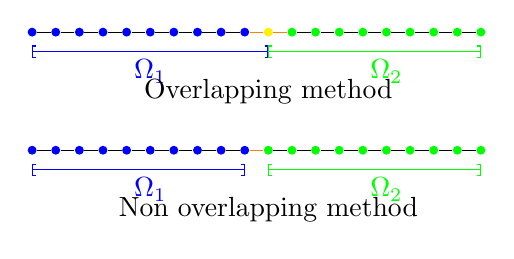
\begin{tikzpicture}
            \foreach \x in { 0,1, ..., 9}
            {
                \node[fill=blue,circle,inner sep=0.4mm] (A\x) at (0.3*\x,0) {};
            }
            \draw (A0) -- (A1);
            \draw (A1) -- (A2);
            \draw (A2) -- (A3);
            \draw (A3) -- (A4);
            \draw (A4) -- (A5);
            \draw (A5) -- (A6);
            \draw (A6) -- (A7);
            \draw (A7) -- (A8);
            \draw (A8) -- (A9);

            \node[fill=yellow,circle,inner sep=0.4mm] (A10) at (3,0) {};

            \foreach \x in { 11,12, ...,19}
            {
                \node[fill=green,circle,inner sep=0.4mm] (A\x) at (0.3*\x,0) {};
            }
            \draw (A11) -- (A12);
            \draw (A12) -- (A13);
            \draw (A13) -- (A14);
            \draw (A14) -- (A15);
            \draw (A15) -- (A16);
            \draw (A16) -- (A17);
            \draw (A17) -- (A18);
            \draw (A18) -- (A19);

            \draw[color=orange] (A9)  -- (A10);
            \draw[color=orange] (A10) -- (A11);

            %\node at (1.5, 0.5) {\textcolor{blue}{$\Omega_{1}$}};
            %\draw[arrows = {-Bracket[reversed,line cap=butt]},color=blue] (0,0.25) -- (3,0.25);
            %\node at (4.5, 0.5) {\textcolor{green}{$\Omega_{2}$}};
            %\draw[arrows = {-Bracket[reversed,line cap=butt]},color=green] (5.7,0.25) -- (3,0.25);
            %\node at (3.0, 0.5) {\textcolor{red}{$\Omega_{3}$}};

            \node at (1.5, -0.5) {\textcolor{blue}{$\Omega_{1}$}};
            \draw[arrows = {Bracket[line cap=butt]-Bracket[line cap=butt]},color=blue] (0,-0.25) -- (3,-0.25);
            \node at (4.5, -0.5) {\textcolor{green}{$\Omega_{2}$}};
            \draw[arrows = {Bracket[line cap=butt]-Bracket[line cap=butt]},color=green] (5.7,-0.25) -- (3,-0.25);

            \node at (3,-0.75) {Overlapping method};
            %%%%%%%%%%%%%%%%%%%%%%%%%%%%%%%%%%%%%%%%%%%%%%%%%%%%%%%%%%%%%
            \foreach \x in { 0,1, ..., 9}
            {
                \node[fill=blue,circle,inner sep=0.4mm] (B\x) at (0.3*\x,-1.5) {};
            }
            \draw (B0) -- (B1);
            \draw (B1) -- (B2);
            \draw (B2) -- (B3);
            \draw (B3) -- (B4);
            \draw (B4) -- (B5);
            \draw (B5) -- (B6);
            \draw (B6) -- (B7);
            \draw (B7) -- (B8);
            \draw (B8) -- (B9);

            \foreach \x in { 10,11,12, ...,19}
            {
                \node[fill=green,circle,inner sep=0.4mm] (B\x) at (0.3*\x,-1.5) {};
            }
            \draw (B10) -- (B11);
            \draw (B11) -- (B12);
            \draw (B12) -- (B13);
            \draw (B13) -- (B14);
            \draw (B14) -- (B15);
            \draw (B15) -- (B16);
            \draw (B16) -- (B17);
            \draw (B17) -- (B18);
            \draw (B18) -- (B19);

            \draw[color=orange] (B9)  -- (B10);

            \node at (1.5, -2.0) {\textcolor{blue}{$\Omega_{1}$}};
            \draw[arrows = {Bracket[line cap=butt]-Bracket[line cap=butt]},color=blue] (0,-1.75) -- (2.7,-1.75);
            \node at (4.5, -2.0) {\textcolor{green}{$\Omega_{2}$}};
            \draw[arrows = {Bracket[line cap=butt]-Bracket[line cap=butt]},color=green] (5.7,-1.75) -- (3.,-1.75);

            \node at (3,-2.25) {Non overlapping method};

        \end{tikzpicture}
    \end{figure}
    \end{multicols}
\end{frame}

\begin{frame}[fragile]{How to split a computing domain ?}
    \scriptsize
    Let $\Omega$ be a rectanglular area in $\mathbb{R}^{2}$.

    Some types of splitting :
    \begin{itemize}
        \item One direction splitting : Easy to care, but not efficiency for communications;
        \item Alternate direction      : Split in two, four or height subdomains the initial domain $\Omega$ and iterate the splitting for subdomains; Harder to care for but more efficient for parallelization and communication;
        \item Adaptive splitting : Anyway, for parallel efficiency, better to split in the direction where we have a minimal number of cells.
    \end{itemize}

    \begin{figure}
        \begin{tikzpicture}
            \draw[fill=yellow,draw] (-4,-2) -- (-2,-2) -- (-2, 1) -- (-4,1) -- cycle;
            \draw[fill=yellow,draw] (-4,-2) grid[xstep=0.1,ystep=0.1] (-2, 1);
            \draw[fill=yellow,draw] (2,-2) -- (0,-2) -- (0, 1) -- (2,1) -- cycle;
            \draw[fill=yellow,draw] (2,-2) grid[xstep=0.1,ystep=0.1] (0, 1);
            \draw[fill=yellow,draw] (4,-2) -- (6,-2) -- (6, 1) -- (4,1) -- cycle;
            \draw[fill=yellow,draw] (4,-2) grid[xstep=0.1,ystep=0.1] (6, 1);

            \only<4>{\draw[color=green,draw,thick] (-3.7,-2) -- (-3.7,1);}
            \only<4>{\draw[color=green,draw,thick] (-3.2,-2) -- (-3.2,1);}
            \only<4>{\draw[color=green,draw,thick] (-2.7,-2) -- (-2.7,1);}
            \only<4>{\draw[color=green,draw,thick] (-2.2,-2) -- (-2.2,1);}
            \only<4>{\draw[color=green,draw,thick] (1.5,-2) -- (1.5,1);}
            \only<4>{\draw[color=green,draw,thick] (0.5,-2) -- (0.5,1);}
            \only<4>{\draw[color=green,draw,thick] (4,-1.2) -- (6,-1.2);}
            \only<4>{\draw[color=green,draw,thick] (4,0.2) -- (6,0.2);}

            \only<3-4>{\draw[color=blue,draw,thick] (-3.5,-2) -- (-3.5,1);}
            \only<3-4>{\draw[color=blue,draw,thick] (-2.5,-2) -- (-2.5,1);}
            \only<3-4>{\draw[color=blue,draw,thick] (2,-0.5) -- (0,-0.5);}
            \only<3-4>{\draw[color=blue,draw,thick] (5,-2) -- (5,1);}

            \only<2-4>{\draw[color=red,draw,thick] (-3,-2) -- (-3,1);}
            \only<2-4>{\draw[color=red,draw,thick] (1,-2) -- (1,1);}
            \only<2-4>{\draw[color=red,draw,thick] (4,-0.5) -- (6,-0.5);}

            \node at (-3,-2.5) {\scriptsize One direction splitting};
            \node at (+1,-2.5) {\scriptsize Alternate direction splitting};
            \node at (+5,-2.5) {\scriptsize Adaptive direction splitting};
        \end{tikzpicture}
    \end{figure}
\end{frame}

\begin{frame}[fragile]{Domain decomposition for non structured mesh}
    \scriptsize

    \begin{multicols}{2}
    \begin{block}{\small Non structured mesh}
        \begin{itemize}
            \item Mesh where cells can't be located with (multi-)indices;
            \item Per example, a triangular mesh
        \end{itemize}
    \end{block}

    \begin{exampleblock}{\small How to split a non structured mesh ?}
        \begin{itemize}
            \item Minimize the size of the interfaces between sub-domains;
            \item Optimal minimization is a NP-problem. 
            \item Use some approximations or heuristics
            \item Some libraries exist for graph partitioning :
            \begin{itemize}
                \item {\scriptsize scotch (Inria);}
                \item {\scriptsize metis (Karypis Lab)};
            \end{itemize}
        \end{itemize}
    \end{exampleblock}

    \begin{figure}[h]
    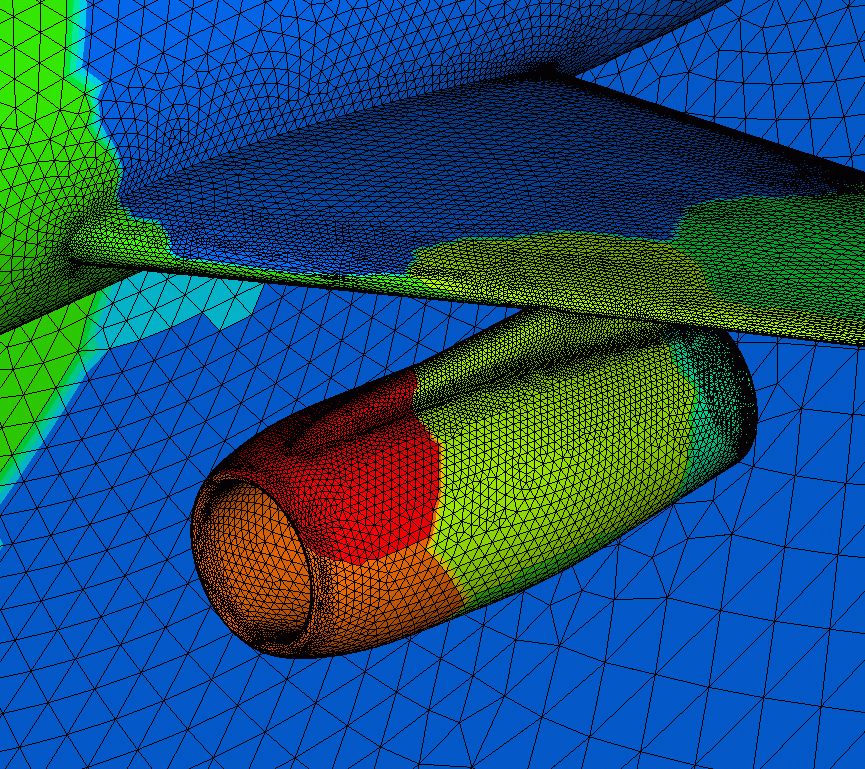
\includegraphics[width=0.40\textwidth]{../Images/grid_decomposition.png}
    \caption{Fun 3D (NASA)}
    \end{figure}
\end{multicols}
\end{frame}

\section{Overlapping domain decomposition methods}



\subsection{Explicit methods}

\begin{frame}[fragile]{Baseline problem}
\scriptsize

\begin{multicols}{2}
\begin{block}{\small Laplacian filter on a gray-scale image}
    \begin{itemize}
        \item A pixel $p_{i,j}$ located by i and j indices on grid
        \item $v_{i,j}$ is the intensity of the pixel $p_{i,j}$;
        \item Discrete Laplacian scheme\\
        $u_{i,j} = v_{i-1,j}+v_{i+1,j}+v_{i,j-1}+v_{i,j+1}-4v_{ij}$
        \item Consider pixel out of the image as black ($=0$)
    \end{itemize}
\end{block}

\begin{figure}
    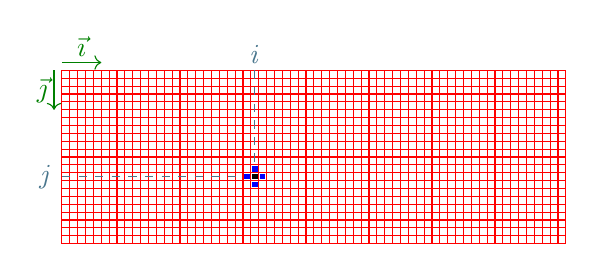
\begin{tikzpicture}
    \draw[color=red] (0,1) grid[step=0.1] (6.4001,3.2001    );        
    \node[fill=black,minimum size=0.1, inner sep=1.0] at (2.45,1.85) {};
    \node[fill=blue,minimum size=0.1, inner sep=1.0] at (2.35,1.85) {};
    \node[fill=blue,minimum size=0.1, inner sep=1.0] at (2.55,1.85) {};
    \node[fill=blue,minimum size=0.1, inner sep=1.0] at (2.45,1.75) {};
    \node[fill=blue,minimum size=0.1, inner sep=1.0] at (2.45,1.95) {};
    \draw[color=DarkGreen, ->] (0,3.3) -- (0.5,3.3) node at (0.25, 3.5) {$\vec{\imath}$};
    \draw[color=DarkGreen, ->] (-0.1,3.2) -- (-0.1,2.7) node at (-0.25,2.95) {$\vec{\jmath}$};
    \draw[color=cyan!50!black, dashed] (2.45, 3.2001) -- (2.45, 2.0) node at (2.45,3.4) {$\mathit{i}$};
    \draw[color=cyan!50!black, dashed] (0, 1.85) -- (2.3, 1.85) node at (-0.2,1.85) {$\mathit{j}$};
    \end{tikzpicture}
\end{figure}
\end{multicols}

\begin{multicols}{2}
\begin{minipage}{0.45\textwidth}
  \begin{figure}
    
\includegraphics[width=0.35\textwidth]{../Images/ned.png}
    \caption{\scriptsize Before filter}
  \end{figure}
\end{minipage}
\begin{minipage}{0.45\textwidth}
  \begin{figure}
    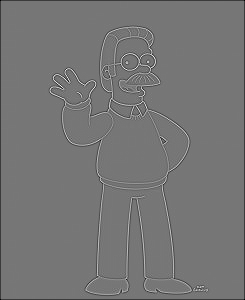
\includegraphics[width=0.35\textwidth]{../Images/lapl_ned.png}
    \caption{\scriptsize After filter}
  \end{figure}
\end{minipage}
\end{multicols}
\end{frame}

\begin{frame}[fragile]{Ghost cells}
  \scriptsize
  \begin{multicols}{2}
  \begin{block}{\small Parallelization of the laplacian filter}
    \begin{itemize}
    \item Apply decomposition domain on image domain;
    \item But need close pixels (right, left, above, bottom);
    \item Add a layer of image pixels in each direction
    \item These pixels are named \textsl{ghost cells};
    \item For sub-domain which contains boundary condition,\\
          fill ghost cells with adequate values.
    \end{itemize}
  \end{block}

  \begin{center}
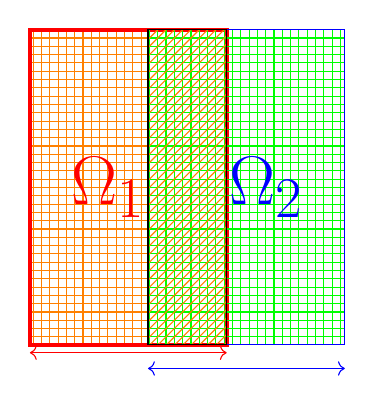
\begin{tikzpicture}
  \draw[color=red, ultra thick, pattern=grid, pattern color=orange] (-2,-2) rectangle (0.5,2);
  \draw[color=blue, pattern=grid, pattern color=green] (-0.5,-2.) rectangle (2,2.);
  \draw[pattern color=orange, pattern = north east lines] (-0.5,-2.) rectangle (0.5,2.);
  \node[color=red] at (-1,0) {\Huge \bf $\Omega_{1}$};
  \node[color=blue] at (1,0) {\Huge \bf $\Omega_{2}$};
  \draw[<->, color=red] (-2,-2.1) -- (0.5,-2.1);
  \draw[<->, color=blue] (-0.5,-2.3) -- (2,-2.3);
  %\draw[ultra thick, loosely dotted,color=orange] (0,0) circle (2cm);
\end{tikzpicture}
\end{center}
\end{multicols}
\end{frame}

\subsection{Implicit methods}

\section{Non overlapping domain decomposition methods}

\subsection{Explicit methods}

\subsection{Implicit methods}

\end{document}
